\documentclass[12pt, xcolor=dvipsnames,svgnames,x11names]{article}
\usepackage{xcolor}
\usepackage{xspace}
\usepackage{url}
\usepackage[colorlinks=true,bookmarks=false,linkcolor=black,urlcolor=blue,citecolor=black]{hyperref}
\usepackage{fancyhdr}
\usepackage[top=1in,bottom=1.2in,left=1in,right=1in]{geometry}
\usepackage{multicol}
\usepackage{pgfplots}
\usepackage{tikz}
\usetikzlibrary{circuits.logic.US, patterns}
\usepackage{mathpazo}
\usepackage{biolinum} 
\usepackage[all]{tcolorbox}
\usepackage{derivative}
\usepackage{../Lectures/rahul_math}
\renewcommand{\familydefault}{\sfdefault}

% --- Custom Color Palette from Image ---
\definecolor{headerRed}{HTML}{A3403D} % Dark red from image top
\definecolor{patternBg}{HTML}{F2D9D7} % Light pinkish bg from image bottom
\definecolor{binaryText}{HTML}{D1A7A4} % Muted color for binary digits

\usepackage{tikz}
\usetikzlibrary{positioning, arrows.meta, shapes.geometric, calc}

% --- Custom Colors ---
\definecolor{lstmBackground}{RGB}{240, 240, 255}
\definecolor{gateGreen}{RGB}{200, 255, 200}
\definecolor{matrixBlue}{RGB}{135, 206, 250}

% --- Background Pattern Setup ---
\usepackage[pages=all]{background}
\backgroundsetup{
scale=1,
color=black,
opacity=1,
angle=0,
contents={%
  \begin{tikzpicture}[remember picture,overlay]
    % Top Header Bar
    \fill[headerRed] (current page.north west) rectangle ([yshift=-1.2cm]current page.north east);
    % Bottom Binary Background
    \fill[patternBg] (current page.south west) rectangle ([yshift=3.5cm]current page.south east);
    % Decorative Line (from image)
    \draw[headerRed, line width=2pt] ([xshift=1in, yshift=-2.5cm]current page.north west) -- ([xshift=8in, yshift=-2.5cm]current page.north west);
    % Binary Text Overlay (Sample)
    \node[anchor=south, binaryText, font=\ttfamily\scriptsize, inner sep=0pt, yshift=1.5cm] at (current page.south) {
        \begin{tabular}{c@{\hspace{0.5em}}c@{\hspace{0.5em}}c@{\hspace{0.5em}}c@{\hspace{0.5em}}c@{\hspace{0.5em}}c@{\hspace{0.5em}}c}
        0 0 0 0 1 1 1 1 0 0 0 0 1 1 0 1 1 1 0 0 0 1 \\
        1 0 0 1 0 1 0 0 0 1 0 0 1 1 0 0 1 0 1 1 \\
        0 0 1 1 0 0 1 0 1 1 1 0 1 1 0 1 0 1 0 0 0 \\
        The University of Alabama in Huntsville
        \end{tabular}
    };
  \end{tikzpicture}
}
}

\newcommand{\hw}{Classwork 04//LSTM}
\newcommand{\duedate}{Feb 19, 2026}

\usetikzlibrary{positioning, arrows.meta, shadows}

% --- Header Styling ---
\makeatletter
\renewcommand{\maketitle}{%
    \vspace*{0.2cm}
    \begin{center}
        \begin{tcolorbox}[
            enhanced,
            colback=white,
            colframe=headerRed,
            arc=0mm,
            title={\textcolor{white}{\bfseries \@title}},
            coltitle=white,
            fonttitle=\bfseries\large,
            attach boxed title to top left={xshift=10pt, yshift=-\tcboxedtitleheight/2},
            boxed title style={sharp corners, colback=headerRed, frame hidden}
        ]
        \large
        \vspace{10pt}
\noindent
\begin{tabular}{@{}p{3.5cm}p{6cm}r@{}}
\textbf{Student Name:} & \underline{\hspace{6cm}} & \textbf{Points:} 30 \\
\end{tabular}

\vspace{10pt}

\noindent
\begin{tabular}{@{}p{3.5cm}p{6cm}r@{}}
\textbf{A Number:} & \underline{\hspace{6cm}} & \textbf{Due Date:} \duedate \\
\end{tabular}
        \end{tcolorbox}
    \end{center}
    \vspace{10pt}
}
\makeatother



\pagestyle{fancy}
\fancyhf{}
\lhead{\small CPE 487/587, Spring 2026}
\rhead{\small \textit{\hw}}
\cfoot{\thepage}
\renewcommand{\headrulewidth}{0pt}

\usepackage{booktabs} % For professional lines


% Define a very light gray for the rows
\definecolor{tablegray}{gray}{0.95}

\begin{document}


\title{\hw}
\maketitle

Assume
\begin{itemize}
\item $W_f , b_f$ weights and bias for the forget gate, $U_f$ weights for recurrent connection for the forget gate.

\item $W_i , b_i$ weights and bias for the input gate, $U_i$ weights for recurrent connection for the input gate.

\item $W_o , b_o$ weights and bias for the output gate, $U_o$ weights for recurrent connection for the output gate.

\item $c_t$ is the cell state or the context vector at time $t$ (like a memory tape).

\item $W_c , b_c$ weights and bias for the cell state, $U_c$ weights for recurrent connection for the cell state.


\end{itemize}


Forget gate operation:

\begin{align*}
f_t = \sigma(W_f x_t + U_f h_{t-1} + b_f)
\end{align*}

Input gate operation:

\begin{align*}
i_i = \sigma(W_i x_t + U_i h_{t-1} + b_i)
\end{align*}

Updated cell state:

\begin{align*}
\tilde{c}_t & = \tanh(W_c x_t + U_c h_{t-1} + b_c)\\
c_t & = f_t \odot c_{t-1} + i_t \cdot \tilde{c}_t
\end{align*}

Output gate:

\begin{align*}
o_t = \sigma(W_o x_t + U_o h_{t-1} + b_o)
\end{align*}

Hidden state:

\begin{align*}
h_t = o_t \odot \tanh(c_t)
\end{align*}


\begin{figure}
\centering
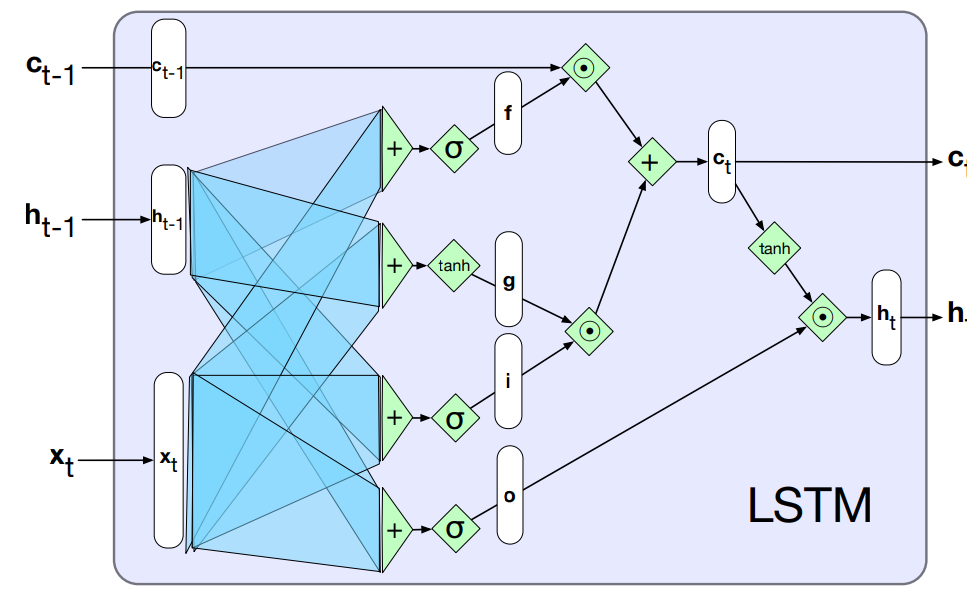
\includegraphics[width=0.7\linewidth]{../Lectures/figures/LSTM_Stanford.png}
\end{figure}

\section{LSTM Output Calculation}

Initial input $x_t = [0.5]$

Previous hidden state $h_{t-1} = [0.2]$

Previous cell state $c_{t-1} = [0.8]$

\begin{enumerate}
\item For the forget gate, consider 
$W_f = [0.5]$, $U_f = [0.3]$, $b_f = 0.0$
Compute the forget gate output $f_t$.



\item For the input gate, consider 
$W_i = [0.6]$, $U_i = [0.4]$, $b_i = 0.0$
Compute the input gate output $i_t$.

\item For the candidate cell, consider 
$W_c = [0.4]$, $U_c = [0.5]$, $b_c = 0.0$
Compute the updated cell state $c_t$.

What percentage of old memory is kept?

What percentage of new candidate is kept?

\item For the output gate, consider 
$W_o = [0.7]$, $U_o = [0.6]$, $b_o = 0.0$
Compute the input gate output $o_t$.

\item Compute the final hidden state $h_t$.
\end{enumerate} 


\subsection{Solution}


\begin{enumerate}
\item \textbf{Forget gate computation:}

$W_f x_t + U_f h_{t-1} + b_f = 0.5\times 0.5 + 0.3 \times 0.2 + 0.0 = 0.31$

$f_t = \frac{1}{1+exp(-0.31)}  = 0.5769$

\item $W_i x_t + U_i h_{t-1} + b_i  = 0.6\times 0.5 + 0.4 \times 0.2 + 0.0 = 0.38$

$i_t = \frac{1}{1+exp(-0.38)}  = 0.5939$

  
\item 

$W_c x_t + U_c h_{t-1} + b_c = 0.4 \times 0.5 + 0.5 \times 0.2 + 0.0 = 0.30$


$\tilde{c}_t = \tanh(0.30)  = 0.2913$

$c_t = 0.5769\times 0.8 + 0.5939\times  0.2913 =  0.4615 + 0.1730 = 0.6345$

Based on $f_t  = 0.5769$, roughly $57.69\%$ of the older memory is kept.

Based on $i_t  = 0.5939$, roughly $59.39\%$ of the new candidate is kept.





\item 

$W_o x_t + U_o h_{t-1} + b_o = 0.7 \times 0.5 + 0.6\times 0.2 + 0.0 = 0.35 + 0.18 = 0.53$ 

$o_t = \frac{1}{1+exp(-0.53)}  = 0.6295$

\item 

$h_t  = 0.6295 \times  \tanh( 0.6345) = 0.3532$.

\end{enumerate}

\end{document}